\documentclass[11pt, a4paper]{article}
\usepackage[a4paper, margin=2.5cm]{geometry}

\usepackage[magyar]{babel}


\usepackage{enumitem}
\setlist[itemize]{label=-}
\usepackage{amsmath}

%%% Megjelenítéshez automatikusan kiegészített csomagok %%%
\usepackage[utf8]{inputenc}
\usepackage[T1]{fontenc}
\usepackage{amssymb, amsfonts, amsthm}
\usepackage{xcolor}
\usepackage{tcolorbox}
\tcbuselibrary{theorems,skins,breakable}
\usepackage{tikz}
\usepackage{pgfplots}
\pgfplotsset{compat=1.18}
\usepackage{graphicx}
\usepackage{booktabs}
\usepackage{float}
\usepackage{caption}
\usepackage{microtype}

\usepackage{hyperref}

\begin{document}

\begin{center}
    \LARGE \textbf{Ismétlés nélküli permutáció} \\
    \vspace{0.5cm}
\end{center}



\vspace{0.5cm}

\subsection*{1. A lényeg}
Képzeld el, hogy van pár teljesen különböző dolgod, és egyszerűen csak sorba akarod rendezni őket. Az \textbf{ismétlés nélküli permutáció} nem más, mint annak a kiszámítása, hogy hányféleképpen állíthatod sorba ezeket a dolgokat úgy, hogy mindegyiket pontosan egyszer használod fel.

\subsection*{2. Miért pont így működik?}
Gondolj arra, hogy van három barát: Anna, Balázs és Csaba, és be akarnak ülni a moziba három egymás melletti székre. Hányféleképpen ülhetnek le? Játsszuk le a dolgot a valóságban:
\begin{itemize}
    \item Az \textbf{első székre} még bárki leülhet a három fiatal közül. Tehát ide \textbf{3} lehetőségünk van.
    \item Tegyük fel, hogy Anna leült. A \textbf{második székre} már csak a maradék két ember (Balázs vagy Csaba) ülhet. Tehát ide \textbf{2} lehetőség maradt.
    \item A \textbf{harmadik székhez} érve már nincs választásunk: aki kimaradt, annak le kell ülnie. Ide már csak \textbf{1} lehetőség maradt.
\end{itemize}

\begin{center}
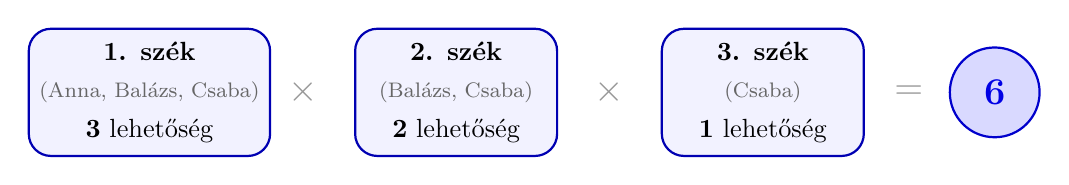
\begin{tikzpicture}[
    scale=0.95,
    every node/.style={transform shape},
    szek/.style={
        draw=blue!70!black,
        fill=blue!5,
        thick,
        rounded corners=8pt,
        align=center,
        minimum width=2.7cm,
        minimum height=1.7cm,
        inner sep=4pt
    },
    muvelet/.style={font=\Large\bfseries, text=gray!80},
    eredmeny/.style={
        draw=blue!80!black,
        fill=blue!15,
        circle,
        thick,
        minimum size=1.2cm,
        font=\Large\bfseries,
        text=blue!90!black
    }
]
    % 1. szék
    \node[szek] (c1) at (0,0) {%
        \textbf{1. szék}\\[2pt]
        {\color{gray!80!black}\footnotesize (Anna, Balázs, Csaba)}\\[3pt]
        \textbf{3} lehetőség
    };

    \node[muvelet] at (2.05,0) {$\times$};

    % 2. szék
    \node[szek] (c2) at (4.1,0) {%
        \textbf{2. szék}\\[2pt]
        {\color{gray!80!black}\footnotesize (Balázs, Csaba)}\\[3pt]
        \textbf{2} lehetőség
    };

    \node[muvelet] at (6.15,0) {$\times$};

    % 3. szék
    \node[szek] (c3) at (8.2,0) {%
        \textbf{3. szék}\\[2pt]
        {\color{gray!80!black}\footnotesize (Csaba)}\\[3pt]
        \textbf{1} lehetőség
    };

    \node[muvelet] at (10.15,0) {$=$};

    % Eredmény
    \node[eredmeny] at (11.3,0) {6};
\end{tikzpicture}
\end{center}

\vspace{0.3em}
\noindent\textbf{Miért szorzunk és miért nem összeadunk?}

A választási lehetőségeket a legkönnyebben egy \textbf{fa-diagrammal} tudjuk szemléltetni. Figyeld meg, hogyan „ágaznak el” a döntések lépésről lépésre:

\begin{center}
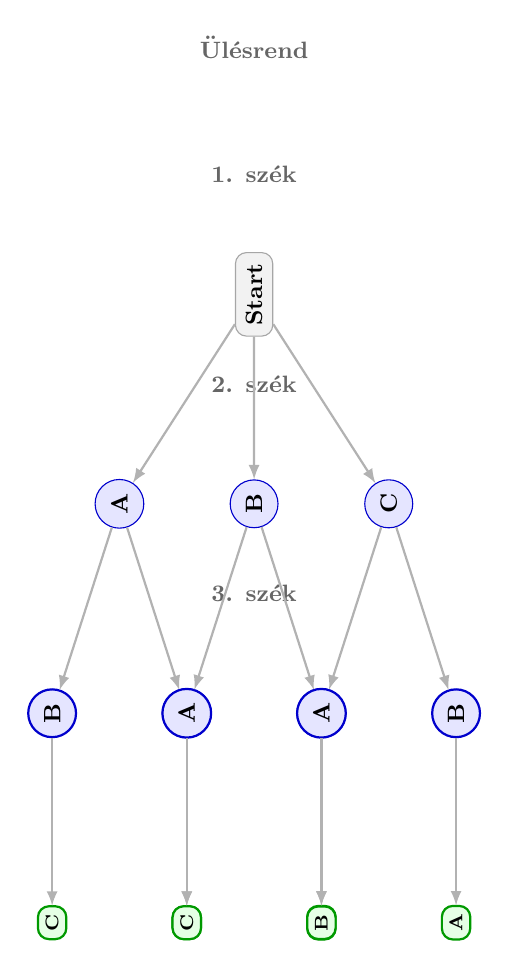
\begin{tikzpicture}[
    scale=0.95, transform shape,
    level 1/.style={sibling distance=18mm, level distance=28mm},
    level 2/.style={sibling distance=18mm, level distance=28mm},
    level 3/.style={sibling distance=18mm, level distance=28mm},
    node_start/.style={rectangle, draw=gray!70, fill=gray!10, rounded corners, font=\bfseries\small, inner sep=4pt},
    node_p/.style={circle, draw=blue!80!black, fill=blue!10, font=\bfseries\small, inner sep=3pt},
    node_end/.style={rectangle, draw=green!60!black, fill=green!10, rounded corners, font=\bfseries\scriptsize, inner sep=3pt},
    edge from parent/.style={draw=gray!60, -latex, thick}
]

% Szintek feliratai a fejlécben
\node[font=\bfseries\small, text=gray!80!black] at (0, 33mm) {Ülésrend};
\node[font=\bfseries\small, text=gray!80!black] at (0, 16mm) {1. szék};
\node[font=\bfseries\small, text=gray!80!black] at (0, -12mm) {2. szék};
\node[font=\bfseries\small, text=gray!80!black] at (0, -40mm) {3. szék};

% Gyökér és ágak (balról jobbra növekedve)
\node[node_start, rotate=90] {Start}
    child { node[node_p, rotate=90] {A}
        child { node[node_p, rotate=90] {B}
            child { node[node_end, rotate=90] {C} }
        }
        child { node[node_p, rotate=90] {C}
            child { node[node_end, rotate=90] {B} }
        }
    }
    child { node[node_p, rotate=90] {B}
        child { node[node_p, rotate=90] {A}
            child { node[node_end, rotate=90] {C} }
        }
        child { node[node_p, rotate=90] {C}
            child { node[node_end, rotate=90] {A} }
        }
    }
    child { node[node_p, rotate=90] {C}
        child { node[node_p, rotate=90] {A}
            child { node[node_end, rotate=90] {B} }
        }
        child { node[node_p, rotate=90] {B}
            child { node[node_end, rotate=90] {A} }
        }
    };
\end{tikzpicture}
\end{center}



Mert ezek a döntések egymásba ágyazódnak, mint egy fa ágai. Bárki is ült az első székre (3 eset), ahhoz a döntéshez \textit{minden alkalommal} 2 újabb eset tartozik a második széknél. A „minden esethez ennyi meg ennyi eset tartozik” a matematikában szorzást jelent. Így a végeredmény: $3 \cdot 2 \cdot 1 = 6$ féle sorrend.

\subsection*{3. Általános képlet és speciális esetek}
Ha nem 3, hanem $n$ darab különböző elemünk van, a logikánk ugyanez marad: elindulunk $n$-től, és egyesével csökkentve összeszorozzuk a számokat 1-ig. Ezt a folyamatot a matematika felkiáltójellel jelöli, amit \textbf{faktoriálisnak} hívunk.

\textbf{Definíció:} $n$ különböző elem egy lehetséges sorrendjét az elemek egy \emph{ismétlés nélküli permutációjának} nevezzük. Az $n$ elem összes lehetséges sorrendjének a száma $P_n$.

$P_n = n! = n \cdot (n - 1) \cdot (n - 2) \cdot \ldots \cdot 1$

\vspace{0.2cm}
\noindent\textbf{Csapdák és határesetek:}
\begin{itemize}
    \item \textbf{Vigyázz, mikor használod!} Ez a képlet szigorúan csak akkor működik, ha az elemek \textbf{különböznek} (nincs két egyforma könyv, golyó, betű, szám stb.). Ha lennének egyformák, akkor osztanunk is kellene, nehogy duplán számoljunk.
    \item \textbf{A nulla faktoriális:} Matematikai (és logikai) megállapodás, hogy $0! = 1$. Hétköznapira lefordítva: ha nulla dolgot kell sorbaraknod, azt pontosan 1-féleképpen teheted meg (üresen hagyod a helyet).
\end{itemize}

\vspace{0.5cm}
\noindent\fbox{
    \begin{minipage}{\dimexpr\textwidth-2\fboxsep-2\fboxrule\relax}
        \vspace{0.2cm}
        \textbf{\large 4. Dolgozat gyorsteszt} \\[0.2cm]
        Amikor a dolgozatban meglátsz egy feladatot, futtasd le ezt a 3 pontos ellenőrzést. Ha mindháromra \textbf{IGEN} a válasz, akkor nyert ügyed van, ez a te képleted ($n!$):
        \begin{enumerate}
            \item \textbf{Ugyanannyi a hely, mint az elem?} (Mindenkit leültetünk? Minden könyvet felrakunk a polcra? Nem marad ki semmi?)
            \item \textbf{Számít a sorrend?} (Anna-Balázs nem ugyanaz, mint Balázs-Anna?)
            \item \textbf{Minden elem különbözik?} (Nincsenek klónok, egyforma színű golyók?)
        \end{enumerate}
        \vspace{0.2cm}
    \end{minipage}
}
\vspace{0.5cm}

\subsection*{5. Tipikus és trükkös feladatok levezetése}

\begin{enumerate}[label=\arabic*., leftmargin=*]
    \item \textbf{Alapfeladat (Sorrend a moziban)}\\
    \textit{Egy 5 fős társaság moziba megy. Hányféleképpen ülhetnek le egymás mellé egy 5 székből álló sorban?}
    \begin{itemize}
        \item \textbf{A gondolatmenet:} Mind az 5 ember különálló elem, és mind az 5 helyre leülnek. Mivel a sorrend számít, ez 5 elem permutációja.
        \item \textbf{A megoldás:} $5! = 5 \cdot 4 \cdot 3 \cdot 2 \cdot 1 = 120$. Tehát 120-féleképpen ülhetnek le.
    \end{itemize}

    \vspace{0.5cm}

    \item \textbf{A "ragasztós" trükk (Összetartozó elemek)}\\
    \textit{Egy 5 fős társaság leül 5 székre, amik egy sorban vannak. Hányféleképpen ülhetnek le, ha Béla és Cili mindenképpen egymás mellett akarnak ülni?}

    \begin{center}
    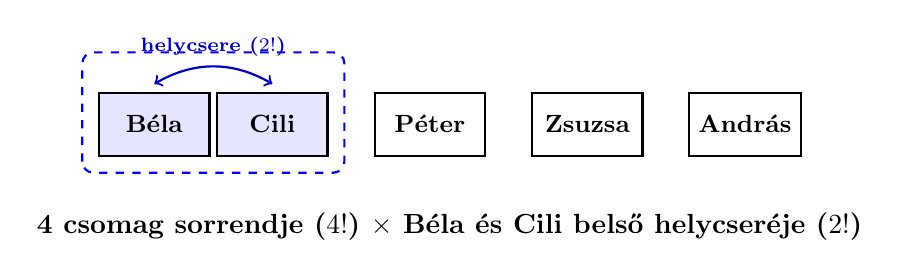
\begin{tikzpicture}[
        box/.style={draw, thick, rectangle, minimum width=1.4cm, minimum height=0.8cm, align=center, font=\small\bfseries}
    ]
        % A 4 logikai "egység" (Béla és Cili egyetlen blokkot alkot)
        \node[box, fill=blue!10] (bela) at (0,0) {Béla};
        \node[box, fill=blue!10] (cili) at (1.5,0) {Cili};
        \node[box] (p1) at (3.5,0) {Péter};
        \node[box] (p2) at (5.5,0) {Zsuzsa};
        \node[box] (p3) at (7.5,0) {András};

        % Kék, szaggatott vonal Béla és Cili körül, jelezve, hogy egy egység
        \draw[blue, thick, dashed, rounded corners] 
            ([xshift=-2mm,yshift=-2mm]bela.south west) rectangle ([xshift=2mm,yshift=5mm]cili.north east);

        % Helycsere jelölése a csomagon belül
        \draw[<->, thick, blue!80!black] ([yshift=1mm]bela.north) to[bend left=30] node[above, font=\scriptsize\bfseries] {helycsere ($2!$)} ([yshift=1mm]cili.north);

        % Magyarázó szöveg az ábra alatt középen
        \node[align=center, font=\bfseries] at (3.75,-1.3) {4 csomag sorrendje ($4!$) $\times$ Béla és Cili belső helycseréje ($2!$)};
    \end{tikzpicture}
    \end{center}

    \begin{itemize}
        \item \textbf{1. lépés – A "csomagok" rendezése:} Bélát és Cilit gondolatban \textbf{összeragasztjuk}, mintha ők egyetlen "csomag" lennének. Így az 5 emberből 4 "csomagunk" lett (3 normál ember + 1 ragasztott páros). Ezt a 4 csomagot $4!$-féleképpen rakhatjuk sorba.
        \item \textbf{2. lépés – FIGYELEM! A belső helycsere:} Sok diák itt megáll, és azt hiszi, $4!$ a végeredmény. \textbf{De ne feledd:} a "ragasztott csomagon" belül Béla és Cili még helyet cserélhetnek (Béla-Cili vagy Cili-Béla), ami újabb $2!=2$ lehetőséget jelent!
        \item \textbf{A hibátlan megoldás:} A külső és belső lehetőségeket össze kell szoroznunk: \textbf{$4! \cdot 2! = 24 \cdot 2 = 48$}. Tehát 48-féleképpen ülhetnek le.
    \end{itemize}

    \vspace{0.4cm}

    \item \textbf{Kizárási feladatok (Egymás mellett nem állható elemek)}\\
    \textit{Hányféleképpen ülhet le 5 ember egy padra úgy, hogy Anna és Béla NEM ülhet egymás mellett?}
    \begin{itemize}
        \item \textbf{1. lépés -- Összes eset megkötés nélkül:} Az 5 ember leültetése korlátozás nélkül $\rightarrow$ $5! = 120$ lehetőség.
        \item \textbf{2. lépés -- Tiltott esetek kiszámítása:} Kiszámoljuk azokat az eseteket (lásd 2. feladat), amikor Anna és Béla egymás mellett ül (blokkképzéssel) $\rightarrow$ $4! \cdot 2! = 48$ lehetőség.
        \item \textbf{3. lépés -- Komplementer kivonás:} Az összes esetből levonjuk a tiltott eseteket $\rightarrow$ $120 - 48 = 72$ megfelelő elrendezés van.
    \end{itemize}

    \begin{center}
    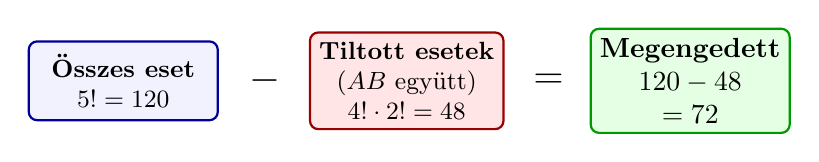
\begin{tikzpicture}[
        card/.style={draw=blue!60!black, fill=blue!5, thick, rounded corners=3pt, minimum width=2.4cm, minimum height=1.0cm, align=center, font=\small},
        forbidden/.style={draw=red!60!black, fill=red!10, thick, rounded corners=3pt, minimum width=2.4cm, minimum height=1.0cm, align=center, font=\small},
        result/.style={draw=green!60!black, fill=green!10, thick, rounded corners=3pt, minimum width=2.4cm, minimum height=1.0cm, align=center, font=\bfseries}
    ]
        \node[card] (c1) at (0,0) {\textbf{Összes eset}\\$5! = 120$};
        \node at (1.8,0) {\Large$-$};
        \node[forbidden] (c2) at (3.6,0) {\textbf{Tiltott esetek}\\$(AB\text{ együtt})$\\$4! \cdot 2! = 48$};
        \node at (5.4,0) {\Large$=$};
        \node[result] (c3) at (7.2,0) {\textbf{Megengedett}\\$120 - 48$\\$= 72$};
    \end{tikzpicture}
    \end{center}

    \vspace{0.4cm}

    \item \textbf{A "korlátozó" feltétel (Fixált helyek)}\\
    \textit{A 0, 1, 2, 3, 4 számjegyekből hány darab 5-jegyű számot tudunk képezni úgy, hogy minden számjegyet pontosan egyszer használunk fel?}
    \begin{itemize}
        \item \textbf{1. lépés – A kritikus hely kiválasztása:} Számoknál mindig bekapcsol a vészvillogó: \textbf{a nulla nem állhat az első helyen}. Ezért az 1. helyre csak az 1, 2, 3, 4 számjegyek kerülhetnek $\rightarrow$ \textbf{4 lehetőség}.
        \item \textbf{2. lépés – A maradék helyek kitöltése:} Mivel az első helyre már leírtunk egy számot, a választható számjegyek száma csökkent, viszont a nulla most már visszakerült a választékba, így ismét 4 számjegy marad a maradék 4 helyre, ami 4 elem sorbarendezése $\rightarrow$ $4!$ lehetőség.
        \item \textbf{3. lépés – A végeredmény kiszámítása:} $4 \cdot 4! = 4 \cdot 24 = 96$ darab ilyen szám van.
    \end{itemize}

    \begin{center}
    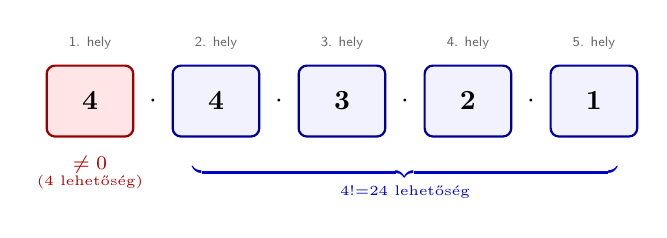
\begin{tikzpicture}[
        box/.style={draw=blue!60!black, fill=blue!5, thick, rounded corners=3pt, minimum width=1.1cm, minimum height=0.9cm, align=center, font=\bfseries},
        firstbox/.style={draw=red!60!black, fill=red!10, thick, rounded corners=3pt, minimum width=1.1cm, minimum height=0.9cm, align=center, font=\bfseries}
    ]
        % 1. hely (korlátozott)
        \node[firstbox] (b1) at (0,0) {4};
        \node[above=2pt, font=\tiny\sffamily, text=gray!80!black] at (b1.north) {1. hely};
        \node[below=3pt, font=\scriptsize, text=red!70!black, align=center] at (b1.south) {$\neq 0$\\[-2pt]\tiny(4 lehetőség)};

        % Műveleti jel
        \node at (0.8,0) {$\cdot$};

        % Maradék helyek
        \node[box] (b2) at (1.6,0) {4};
        \node[above=2pt, font=\tiny\sffamily, text=gray!80!black] at (b2.north) {2. hely};

        \node at (2.4,0) {$\cdot$};

        \node[box] (b3) at (3.2,0) {3};
        \node[above=2pt, font=\tiny\sffamily, text=gray!80!black] at (b3.north) {3. hely};

        \node at (4.0,0) {$\cdot$};

        \node[box] (b4) at (4.8,0) {2};
        \node[above=2pt, font=\tiny\sffamily, text=gray!80!black] at (b4.north) {4. hely};

        \node at (5.6,0) {$\cdot$};

        \node[box] (b5) at (6.4,0) {1};
        \node[above=2pt, font=\tiny\sffamily, text=gray!80!black] at (b5.north) {5. hely};

        % Összefogó kapocs a maradék helyekhez
        \node[below=6pt, font=\scriptsize, text=blue!80!black, align=center] at (4.0,-0.45) {$\underbrace{\hspace{5.4cm}}_{4! = 24\text{ lehetőség}}$};
    \end{tikzpicture}
    \end{center}

    \vspace{0.4cm}

    \item \textbf{Ciklikus / Körmutáció}\\
    \textit{Hányféleképpen ülhet le 5 ember egy kerek asztal köré, ha a forgatással egymásba átvihető ülésrendek azonosnak számítanak?}
    \begin{itemize}
        \item \textbf{1. lépés -- Vonatkoztatási pont rögzítése:} Egy embert rögzítünk az asztalnál (a forgási szimmetria megtöréséhez) $\rightarrow$ \textbf{1 lehetőség}.
        \item \textbf{2. lépés -- Maradék pozíciók kitöltése:} A fennmaradó $(n-1) = 4$ embert a rögzített személyhez képest permutáljuk $\rightarrow$ \textbf{$4!$ lehetőség}.
        \item \textbf{3. lépés -- A végeredmény kiszámítása:} $(5-1)! = 4! = 24$ különböző körültetés létezik.
    \end{itemize}

    \begin{center}
    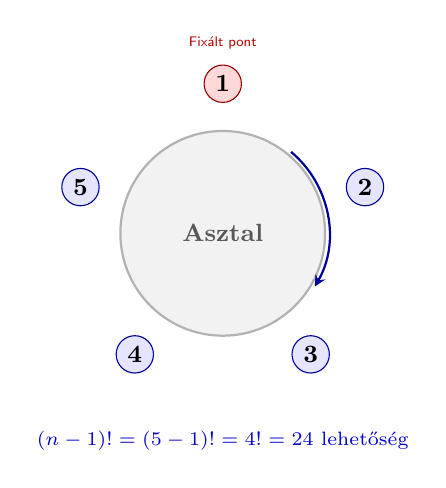
\begin{tikzpicture}
        % Asztal
        \draw[thick, fill=gray!10, draw=gray!60] (0,0) circle (1.3cm);
        \node[font=\small\bfseries, text=gray!70!black] at (0,0) {Asztal};

        % Székek / Elemek
        \node[draw=red!60!black, fill=red!15, circle, inner sep=2pt, font=\bfseries\small] (p1) at (90:1.9cm) {1};
        \node[above=2pt, font=\tiny\sffamily, text=red!70!black] at (p1.north) {Fixált pont};

        \node[draw=blue!60!black, fill=blue!10, circle, inner sep=2pt, font=\bfseries\small] (p2) at (18:1.9cm) {2};
        \node[draw=blue!60!black, fill=blue!10, circle, inner sep=2pt, font=\bfseries\small] (p3) at (306:1.9cm) {3};
        \node[draw=blue!60!black, fill=blue!10, circle, inner sep=2pt, font=\bfseries\small] (p4) at (234:1.9cm) {4};
        \node[draw=blue!60!black, fill=blue!10, circle, inner sep=2pt, font=\bfseries\small] (p5) at (162:1.9cm) {5};

        % Forgási nyíl
        \draw[->, >=stealth, thick, blue!60!black] (50:1.35cm) arc (50:-30:1.35cm);
        
        % Képlet
        \node[below=14pt, font=\scriptsize, text=blue!80!black, align=center] at (0,-1.9cm) {$(n-1)! = (5-1)! = 4! = 24\text{ lehetőség}$};
    \end{tikzpicture}
    \end{center}

    \vspace{0.4cm}

    \item \textbf{Kötött / Rögzített pozíciók}\\
    \textit{Hányféleképpen futhat be 6 versenyző a célba, ha a leggyorsabb futó (A) biztosan az 1. helyen végez?}
    \begin{itemize}
        \item \textbf{1. lépés -- A rögzített pozíció rögzítése:} Az 1. helyre csak az A futó kerülhet $\rightarrow$ \textbf{1 lehetőség}.
        \item \textbf{2. lépés -- A maradék helyek kitöltése:} A 2.--6. helyekre a maradék 5 futó tetszőleges sorrendben érkezhet $\rightarrow$ \textbf{$5!$ lehetőség}.
        \item \textbf{3. lépés -- A végeredmény kiszámítása:} $1 \cdot 5! = 1 \cdot 120 = 120$ befutási sorrend létezik.
    \end{itemize}

    \begin{center}
    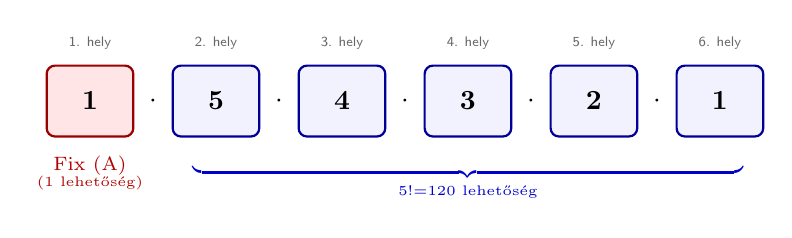
\begin{tikzpicture}[
        box/.style={draw=blue!60!black, fill=blue!5, thick, rounded corners=3pt, minimum width=1.1cm, minimum height=0.9cm, align=center, font=\bfseries},
        fixbox/.style={draw=red!60!black, fill=red!10, thick, rounded corners=3pt, minimum width=1.1cm, minimum height=0.9cm, align=center, font=\bfseries}
    ]
        \node[fixbox] (b1) at (0,0) {1};
        \node[above=2pt, font=\tiny\sffamily, text=gray!80!black] at (b1.north) {1. hely};
        \node[below=3pt, font=\scriptsize, text=red!70!black, align=center] at (b1.south) {Fix (A)\\[-2pt]\tiny(1 lehetőség)};

        \node at (0.8,0) {$\cdot$};

        \node[box] (b2) at (1.6,0) {5};
        \node[above=2pt, font=\tiny\sffamily, text=gray!80!black] at (b2.north) {2. hely};

        \node at (2.4,0) {$\cdot$};

        \node[box] (b3) at (3.2,0) {4};
        \node[above=2pt, font=\tiny\sffamily, text=gray!80!black] at (b3.north) {3. hely};

        \node at (4.0,0) {$\cdot$};

        \node[box] (b4) at (4.8,0) {3};
        \node[above=2pt, font=\tiny\sffamily, text=gray!80!black] at (b4.north) {4. hely};

        \node at (5.6,0) {$\cdot$};

        \node[box] (b5) at (6.4,0) {2};
        \node[above=2pt, font=\tiny\sffamily, text=gray!80!black] at (b5.north) {5. hely};

        \node at (7.2,0) {$\cdot$};

        \node[box] (b6) at (8.0,0) {1};
        \node[above=2pt, font=\tiny\sffamily, text=gray!80!black] at (b6.north) {6. hely};

        \node[below=6pt, font=\scriptsize, text=blue!80!black, align=center] at (4.8,-0.45) {$\underbrace{\hspace{7.0cm}}_{5! = 120\text{ lehetőség}}$};
    \end{tikzpicture}
    \end{center}

    \item \textbf{Váltakozó / Paritásos elrendezések}\\
    \textit{Hányféleképpen ülhet le 3 fiú (F) és 3 lány (L) egy 6 székes sorba úgy, hogy fiú és lány felváltva üljön?}
    \begin{itemize}
        \item \textbf{1. lépés -- Mintázat kiválasztása:} Két lehetséges szerkezet van: F--L--F--L--F--L vagy L--F--L--F--L--F $\rightarrow$ \textbf{2 lehetőség}.
        \item \textbf{2. lépés -- Személyek permutációja:} A 3 fiú a saját helyein $3!$-féleképpen, a 3 lány a saját helyein $3!$-féleképpen cserélhet helyet.
        \item \textbf{3. lépés -- A végeredmény kiszámítása:} $2 \cdot 3! \cdot 3! = 2 \cdot 6 \cdot 6 = 72$ ültetési rend lehetséges.
    \end{itemize}

    \begin{center}
    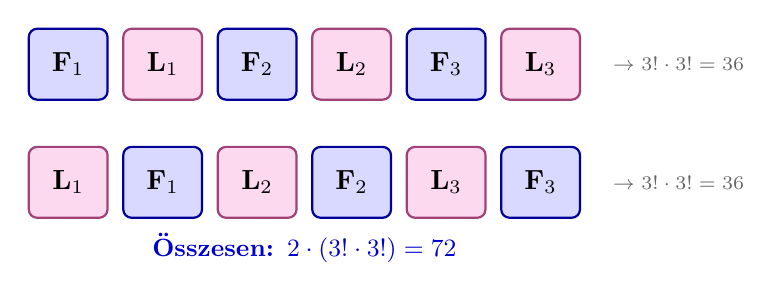
\begin{tikzpicture}[
        boy/.style={draw=blue!60!black, fill=blue!15, thick, rounded corners=3pt, minimum width=1.0cm, minimum height=0.9cm, align=center, font=\bfseries},
        girl/.style={draw=magenta!60!black, fill=magenta!15, thick, rounded corners=3pt, minimum width=1.0cm, minimum height=0.9cm, align=center, font=\bfseries}
    ]
        % Első sor: F1 L1 F2 L2 F3 L3
        \node[boy] (b1) at (0,0) {F$_1$};
        \node[girl] (g1) at (1.2,0) {L$_1$};
        \node[boy] (b2) at (2.4,0) {F$_2$};
        \node[girl] (g2) at (3.6,0) {L$_2$};
        \node[boy] (b3) at (4.8,0) {F$_3$};
        \node[girl] (g3) at (6.0,0) {L$_3$};

        \node[right=8pt, font=\scriptsize, text=gray!80!black] at (g3.east) {$\rightarrow 3! \cdot 3! = 36$};

        % Második sor: L1 F1 L2 F2 L3 F3 (normál méretben)
        \node[girl] (ig1) at (0,-1.5) {L$_1$};
        \node[boy] (ib1) at (1.2,-1.5) {F$_1$};
        \node[girl] (ig2) at (2.4,-1.5) {L$_2$};
        \node[boy] (ib2) at (3.6,-1.5) {F$_2$};
        \node[girl] (ig3) at (4.8,-1.5) {L$_3$};
        \node[boy] (ib3) at (6.0,-1.5) {F$_3$};

        \node[right=8pt, font=\scriptsize, text=gray!80!black] at (ib3.east) {$\rightarrow 3! \cdot 3! = 36$};

        % Összesen felirat
        \node[below=15pt, font=\bfseries\small, text=blue!80!black] at (3.0,-1.5) {Összesen: $2 \cdot (3! \cdot 3!) = 72$};
    \end{tikzpicture}
\end{center}

\end{enumerate}


\end{document}